\chapter{Koncepcja systemu śledzenia obiektów}
\label{sec:koncepcja}

Realizacja projektu śledzenia obiektów dla potrzeb nawigacji bezzałogowego statku powietrznego dotyczy detekcji osoby w postawie stojącej. Na podstawie analizy obrazu wideo powinna być określona pozycja osoby względem drona, a w wyniku tego realizowane sterowanie, mające na celu utrzymać platformę w zadanej pozycji. Rysunek \ref{fig:tracking_scheme} przedstawia ideę takiego systemu.
\begin{figure}[h]
	\centering
	\captionsetup{justification=centering,margin=1cm}
	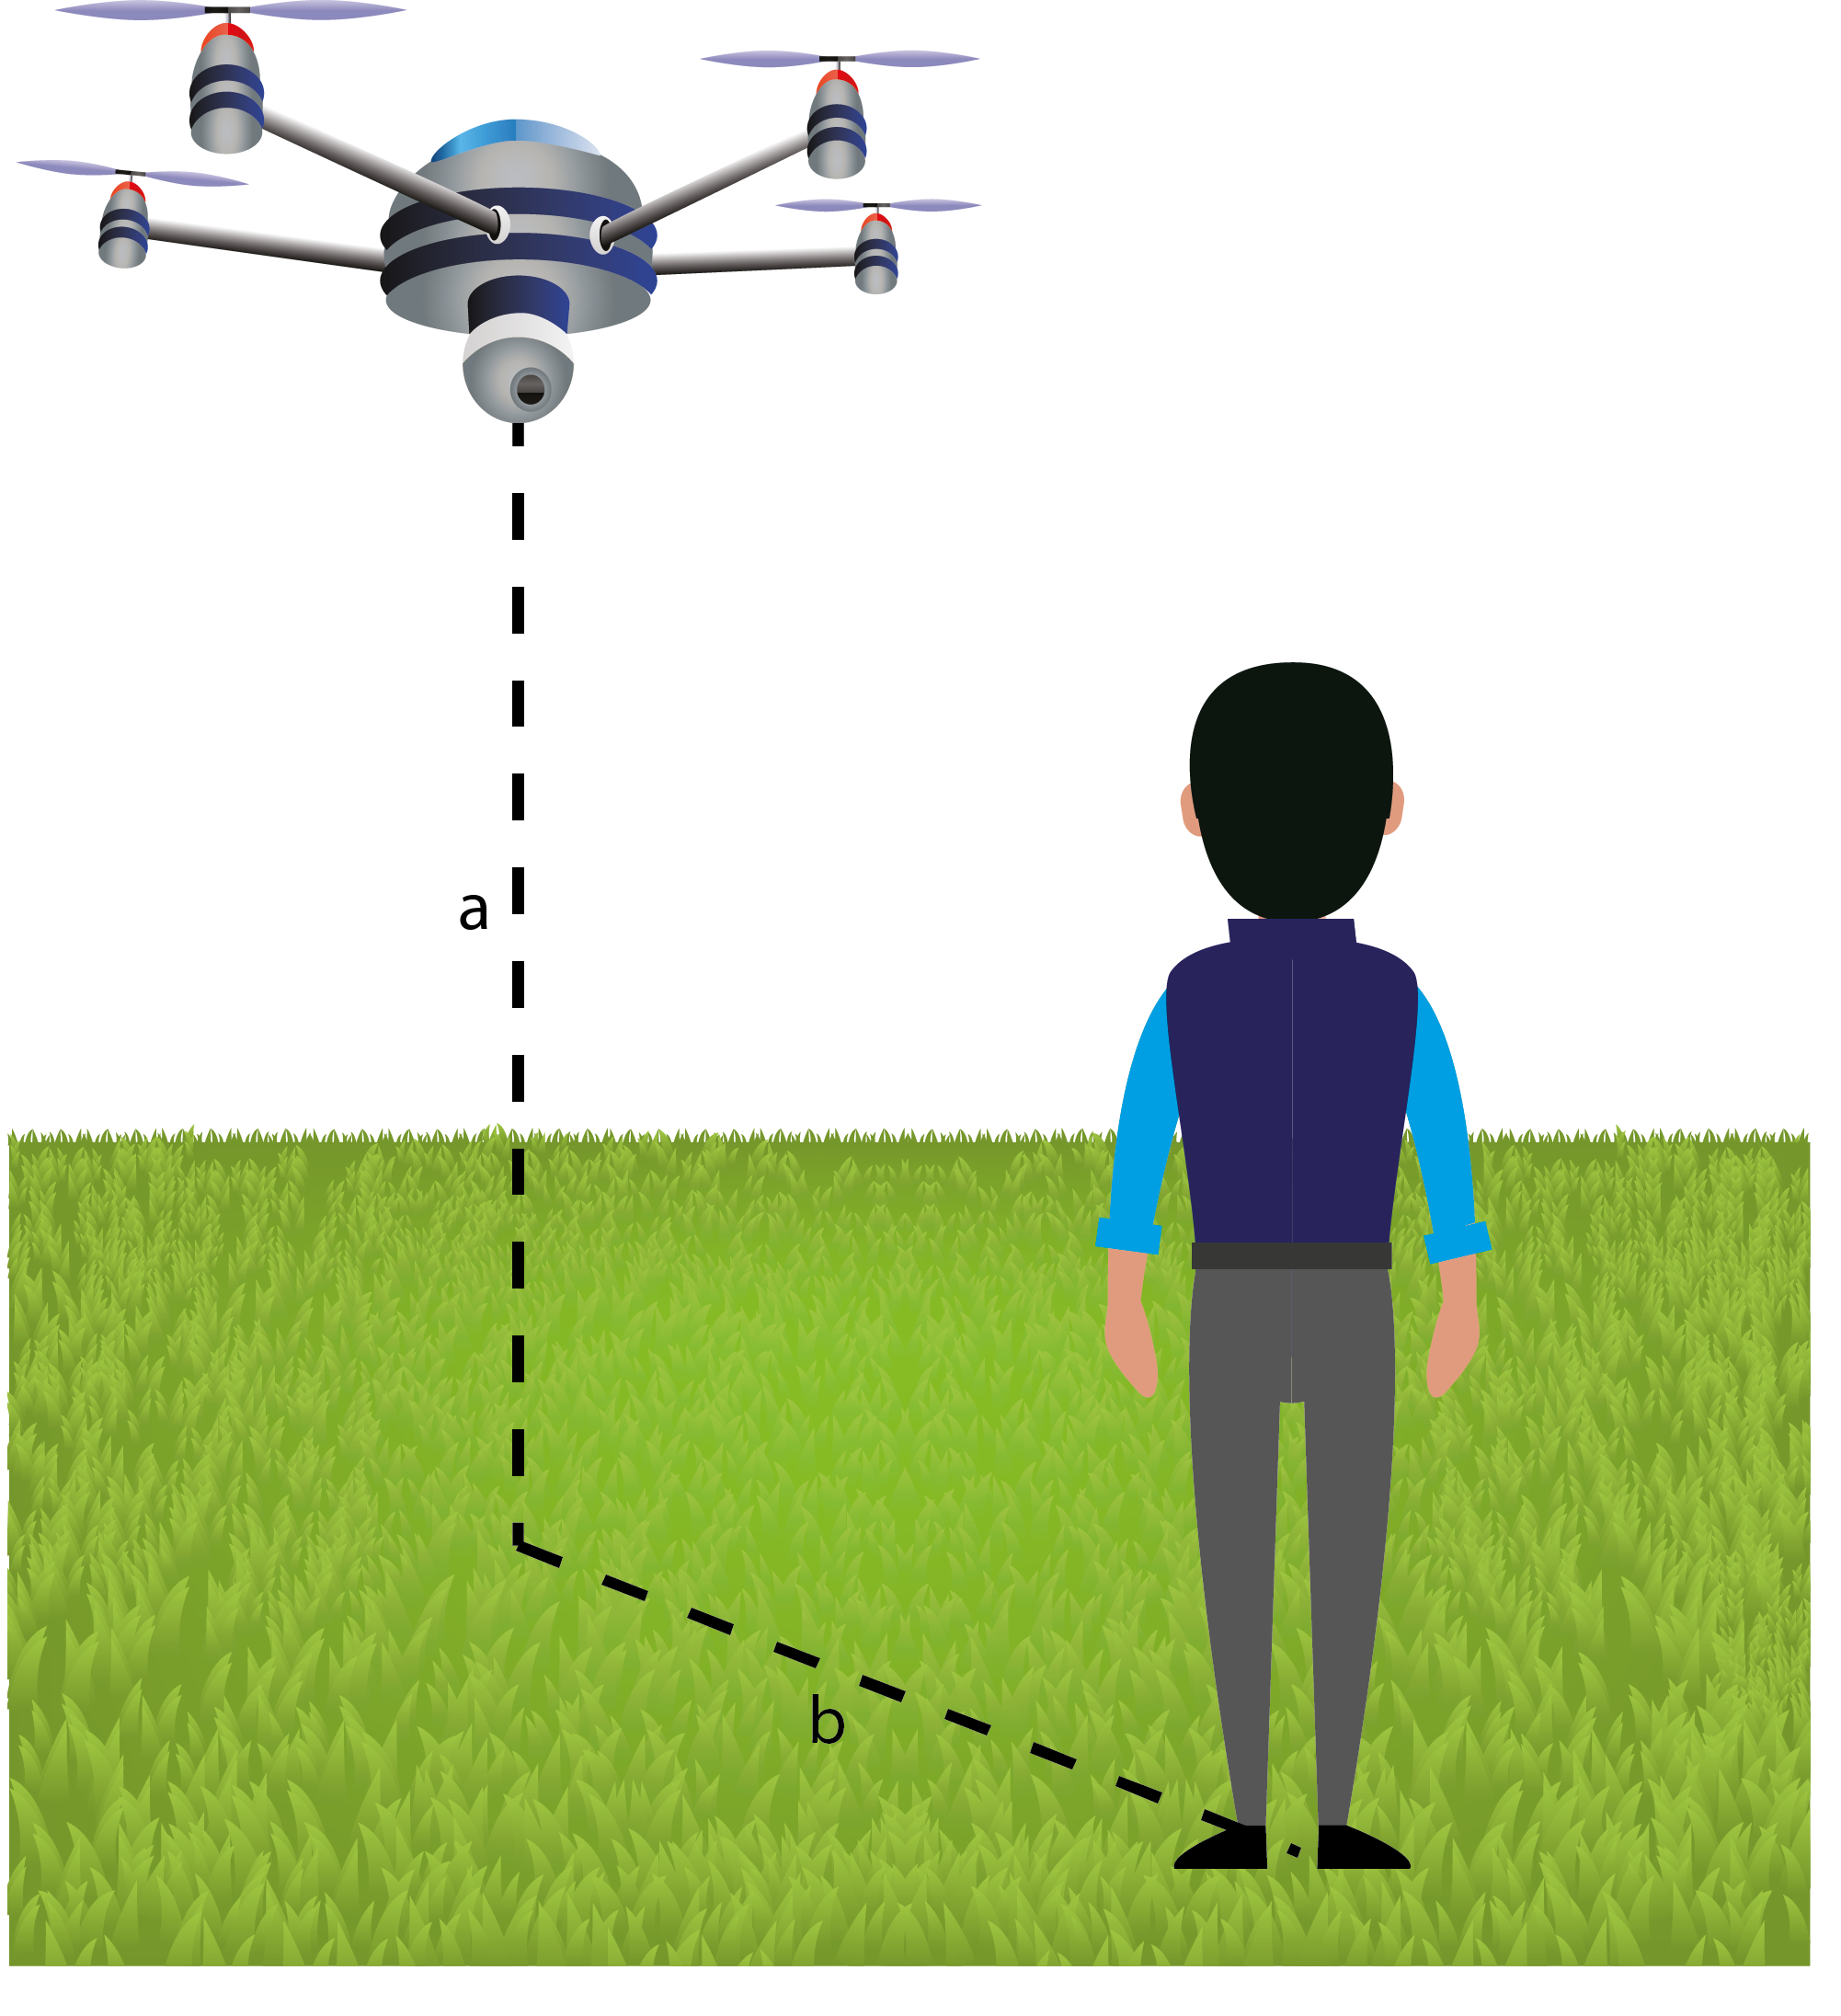
\includegraphics[width=10cm]{tracking_scheme.png}
	\caption{Śledzenie osoby realizowane przez platformę UAV}
	\label{fig:tracking_scheme}
\end{figure}

%TODO 2 tu jednak szerszy opis, moze rysunek poglądaowy (dron, ludzik te Pana parametry..). Bo to zadnie nie oddaje problemu.
Wymagane było tu zdefiniowanie kilku założeń:
\begin{itemize}
	\item detekcja osoby znajdującej się jedynie w bezpośrednim otoczeniu drona, wewnątrz okręgu o promieniu do 7 metrów
	\item śledzenie poprzez ruch całej platformy -- kamera jest nieruchoma, a jej pozycję dodatkowo stabilizuje gimbal kompensując wychylenia drona,
	\item śledzenie w przestrzeni trójwymiarowej, z zadaną pozycją:
	\begin{itemize}
		\item wysokość $a$: około $1.5$m od ziemi
		\item odległość $b$: około $4$m od osoby
		\item przesunięcie względem osoby $c$: $0$m, tj. osoba powinna znajdować się w centrum obrazu rejestrowanego przez kamerę		
	\end{itemize} 
	\item automatyzacja misji -- do zadań użytkownika należy jedynie wydanie rozkazu startu z~ ziemi i zakończenia pracy, skutkującego lądowaniem
	\item możliwość awaryjnego przejęcia manualnej kontroli nad dronem
	\item brak funkcjonalności, która zachowałoby ciągłość detekcji w przypadku pojawienia się drugiej osoby w otoczeniu głównego celu
\end{itemize}


Dodatkowym warunkiem było oparcie prac na konstrukcji opisanej w kolejnych podrozdziałach.

\section{Platforma UAV}
Platforma, na której realizowany jest projekt, składa się z następujących elementów:
\begin{itemize}
	\item typ obiektu: hexacopter (rama DJI F550),
	\item rodzaj śmigieł: wzmocnione śmigła o oznaczeniu 9050, czyli o średnicy śmigła równej $9.0"$ ($~22.86$cm) oraz skoku śmigła $5.0"$ ($~12.7$cm).,
	\item silniki: DJI 2312/960KV sterowane kontrolerami 420 LITE,
	\item zasilanie: czterokomorowa bateria LiPo o nominalnym napięciu $14.8$V (maksymalnym $16.8$V) oraz o pojemności $6450$mAh,
	\item kamera: Xiaomi Yi,
	\item gimbal: Tarot T-2D,
	\item aparatura radiowa: FrSky Taranis X9D Plus,
	\item odbiornik: FrSky X8D,
	\item autopilot: 3DR Pixhawk.
    \item platforma obliczeniowa: karta PYNQ z układem Zynq 7Z020.
\end{itemize}
%TODO 2 a nie dodać tutaj PYNQ jako platfomry obliczeniowej - potem Pan to wymienia %ODP OK

Wybór komponentów, montaż platformy i jej kalibracja były częścią tej pracy i w ramach projektu SKN AVADER były dofinansowane ze środków Grantu Rektorskiego AGH 2015 oraz funduszy wydziału EAIiIB.

\section{Autopilot}

Każdy dron byłby bezużyteczną konstrukcją, gdyby nie serce maszyny -- tzw. autopilot. 
W~tym przypadku postanowiono wykorzystać urządzenie Pixhawk. 
Jest to zgodny ze standardami przemysłowymi moduł na otwartej licencji, stworzony przy współpracy z firmą 3D Robotics oraz ArduPilot Group. 
Posiada następujące parametry:
\begin{itemize}
	\item procesor Cortex-M4F taktowany zegarem 168 MHz,
	\item sensory: trzyosiowy akcelerometr, żyroskop, kompas magnetyczny, barometr i zewnętrzny GPS,
	\item slot na kartę microSD,
	\item możliwość połączenia peryferiów (interfejsy: UART, I2C, CAN),
	\item 14 wyjść PWM (8 głównych z zabezpieczeniami + 6 dodatkowych).
\end{itemize}

\begin{figure}[h]
	\centering
	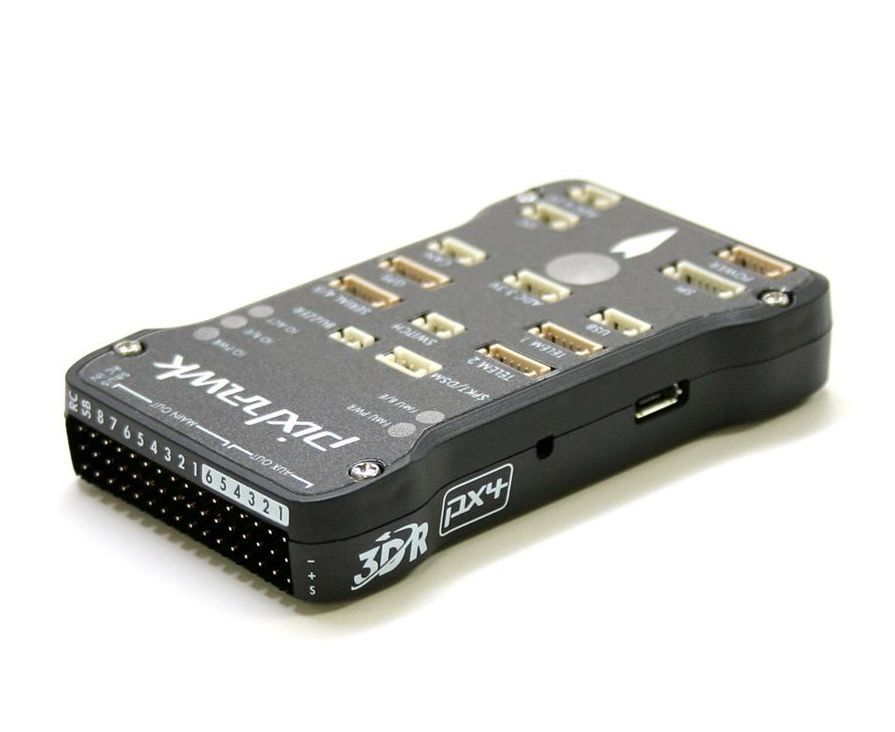
\includegraphics[width=8cm]{5_pixhawk.jpg}
	\caption{Autopilot Pixhawk -- widok na panel główny oraz we/wy PWM}
	\label{fig:pixhawk}
\end{figure}

Powyższy sprzęt jednak nie jest w pełni skonfigurowany do pracy po wyjęciu z pudełka -- szczególnie, że jako produkt uniwersalny, bywa montowany na konstrukcjach o szerokim rozrzucie parametrów. 
Może zapewnić sterowanie śmigłowcom (tzw. multicopterom), samolotom modelarskim oraz nawet łazikom. 
W przypadku dwóch pierwszych grup konfiguracja wiąże się ze zdefiniowaniem odpowiedniej liczby śmigieł i ich rozstawienia, typu aparatury radiowej oraz zewnętrznych urządzeń geolokalizacyjnych. 
Tę dość dużą elastyczność mogą zapewnić dwa główne systemy, które są wczytywane z pamięci SD i pracują w czasie rzeczywistym. 
Dedykowany, PX4 Flight Stack jest stworzony przez twórców modułu, oraz ArduPilot Copter (ArduCopter) -- niezależny, otwarty system, który został dostosowany do platformy Pixhawk z~wykorzystaniem dostępnych narzędzi deweloperskich. 
Ze względu na większą bazę użytkowników i dojrzałość projektu, wybrano drugie rozwiązanie.

\section{Integracja urządzeń na platformie UAV} 

Zbudowanie drona w oparciu o gotowe komponenty nie jest zadaniem skomplikowanym. 
Jednak z uwagi na wymagania projektu (opisane w \ref{sec:koncepcja}), należało dokładnie przemyśleć jego rozbudowę o układ PYNQ, zapewnienie zasilania i montaż na konstrukcji.  %TODO 2 - dlaczego przebudowę ? jesli dodanie tego PYNQ ? %ODP OK, rozbudowę - odpowied
Rysunek \ref{fig:drone_photo} przedstawia zdjęcie zmodyfikowanej, gotowej do lotu platformy.
Z kolei schemat \ref{fig:architecture} opisuje połączenia pomiędzy urządzeniami na platformie UAV.
\begin{figure}[h]
	\centering
	\captionsetup{justification=centering,margin=1cm}
	\hspace*{0cm}
	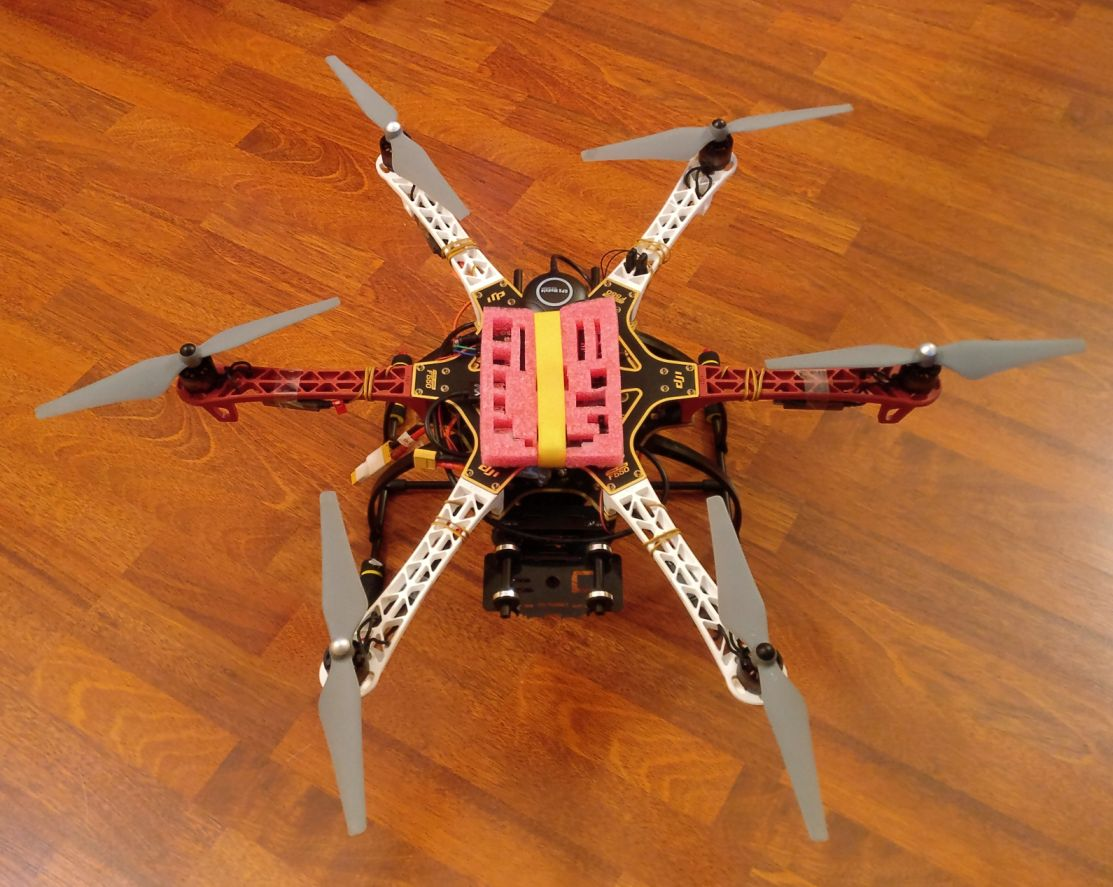
\includegraphics[width=14cm]{5_drone_photo.jpg}
	\caption{Dron po niezbędnych modyfikacjach. Pod gąbką ochronną znajduje się układ PYNQ}
	\label{fig:drone_photo}
\end{figure}
\begin{figure}[]
	\centering
	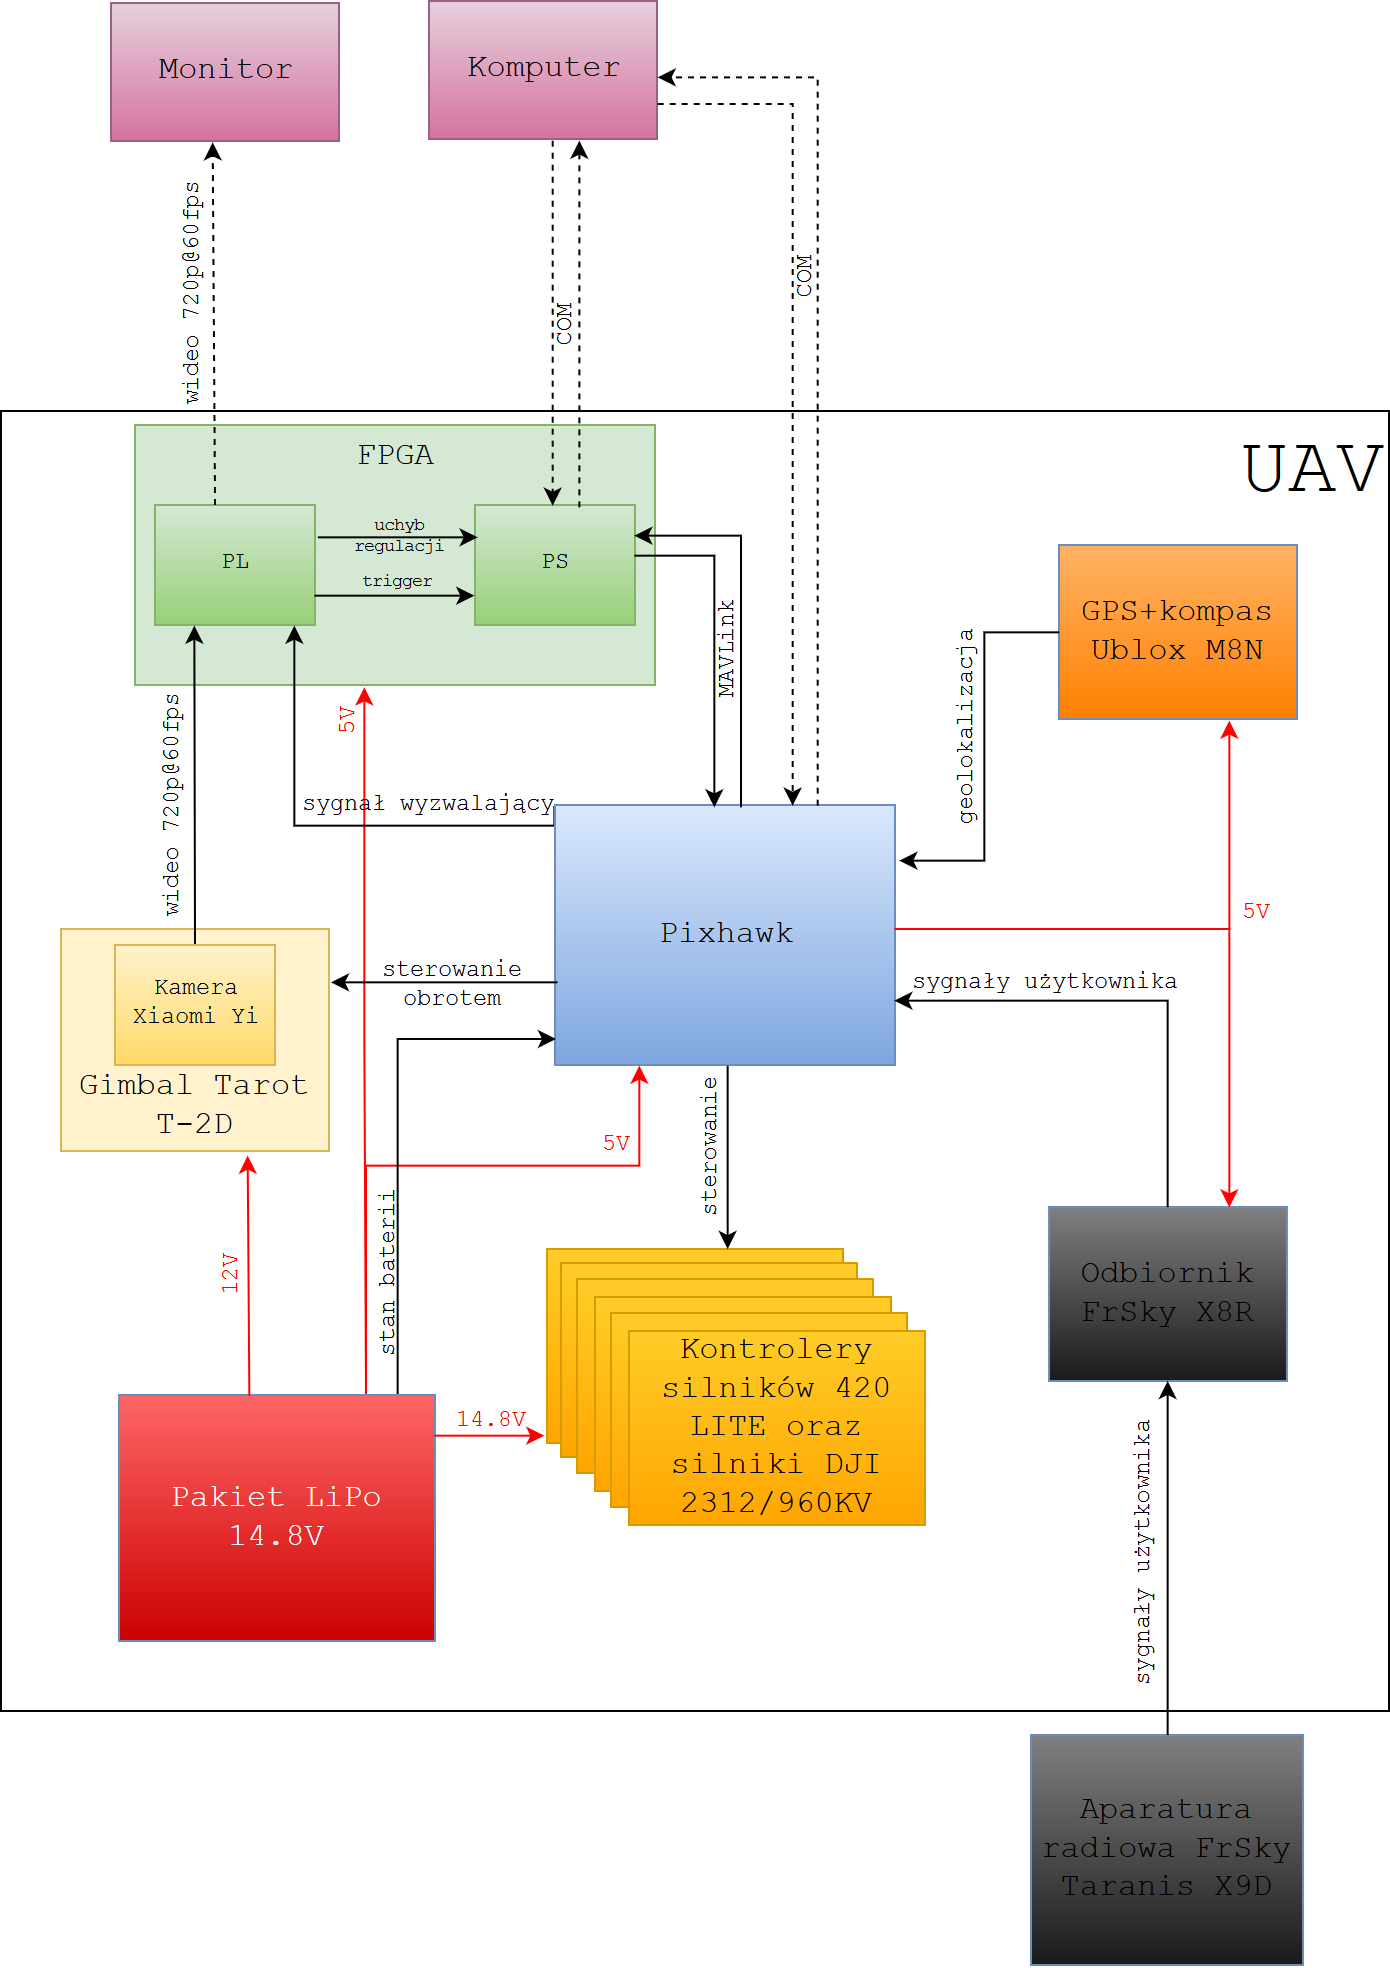
\includegraphics[width=15cm]{5_drone_architecture.png}
	\caption{Relacje pomiędzy urządzeniami na platformie UAV}
	\label{fig:architecture}
\end{figure}
%TODO No to tu nie FPGA, a Zynq %ODP OK
Linie czerwone określają dystrybucję zasilania z~zamontowanej baterii (pominięto konwertery napięcia), natomiast linie czarne opisują propagację sygnałów pomiędzy urządzeniami. 
Dodatkowo, liniami przerywanymi zaznaczono sygnały opcjonalne wykorzystywane w trakcie naziemnej analizy systemu. 
Porty szeregowe komputera służą do komunikacji z konsolą zaimplementowaną na układzie Zynq, oraz do konfiguracji autopilota poprzez aplikację MISSION Planner.






